\documentclass[journal]{IEEEtran}

\usepackage{cite}
\usepackage{amsmath}
\usepackage{verbatim}
\usepackage{multirow}
\usepackage[unicode,pdftex]{hyperref}

\usepackage{xcolor}


\ifCLASSINFOpdf
\usepackage[pdftex]{graphicx}
\else
\fi

\hyphenation{op-tical net-works semi-conduc-tor}

\newcommand{\reffig}[1]{Fig. \ref{#1}}
\newcommand{\refsec}[1]{Section \ref{#1}}
\newcommand{\refeq}[1]{Eq. \ref{#1}}
\newcommand{\reftab}[1]{Table \ref{#1}}

\newcommand{\tabincell}[2]{\begin{tabular}{@{}#1@{}}#2\end{tabular}}

\DeclareMathOperator*{\argmax}{argmax}
\DeclareMathOperator*{\argmin}{argmin}


\definecolor{level2}{RGB}{255,255,255}
\definecolor{level3}{RGB}{10,10,10}
\definecolor{revised}{RGB}{100,101,140}
\definecolor{continue}{RGB}{255,0,0}
\definecolor{filltext}{RGB}{0,255,255}

\begin{document}


\section{Experiments}

\subsection{Evaluation Metric and Dataset}

\begin{equation}
    F=\frac{precision \dot recall}{precision - recall}
\end{equation}
\begin{figure}[!t]	% FIGURE: figure/fig1 
\centering
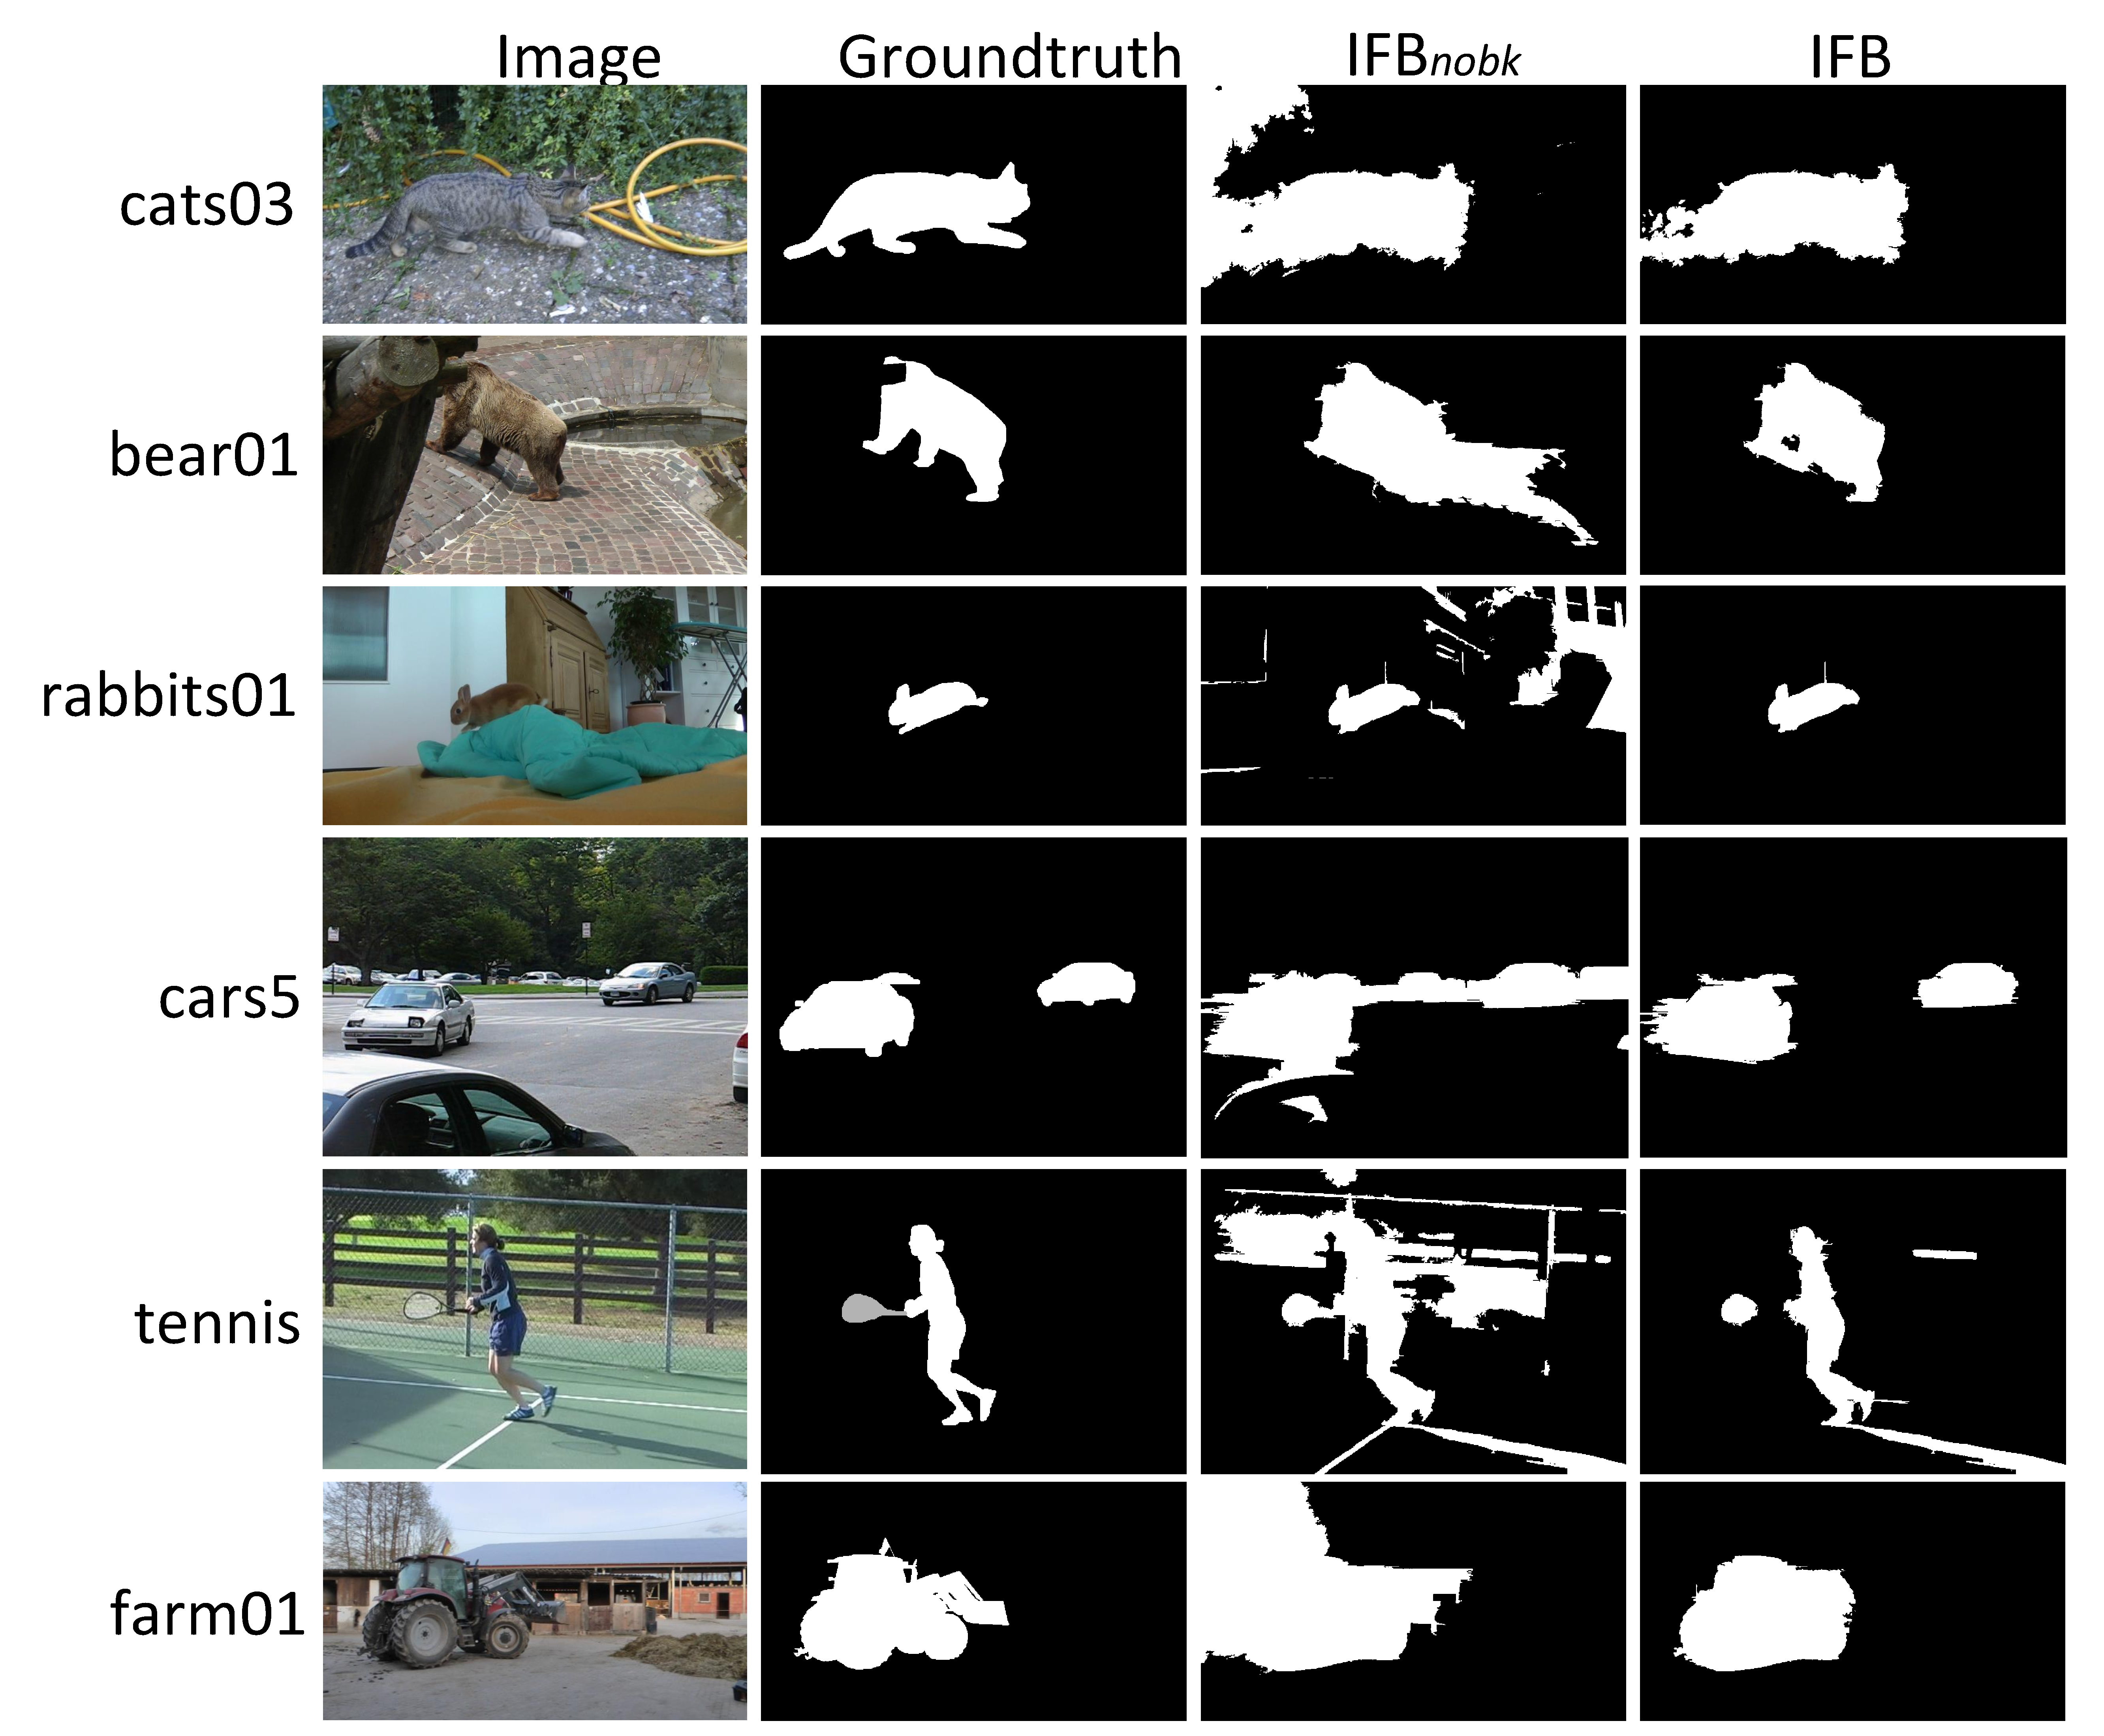
\includegraphics[width=.5\textwidth]{figure/fig_roc_fg}
\DeclareGraphicsExtensions.
    \caption{The example of latex figure.}
\label{fig_FBMS_nobk}
\end{figure}

\begin{table}[!t]				% TABLE
    \caption{The example of latex table}
\label{tab_FBMS_nobk}
\centering
    \begin{tabular}{|l@{  }c@{  }c@{  }cc@{  }c@{  }c@{  }c|}
\hline
     \multirow{2}{*}{Videos} & \multicolumn{3}{c}{$\text{IFB}_{nobk}$} &  & \multicolumn{3}{c|}{IFB} \\
    \cline{2-4} \cline{6-8}
       & Re &Pr & Fm &  &  Re & Pr & Fm  \\
\hline
cats03          &   (\textbf{0.9472} ,\   &  0.5428 ,\  &   0.6901 )   &  &    (0.9063 ,\	 &  \textbf{0.7955} ,\	 &  \textbf{0.8473} )   \\
bear01          &   (\textbf{0.9854} ,\   &  0.4806 ,\  &   0.6461 )   &  &    (0.8695 ,\	 &  \textbf{0.8673} ,\	 &  \textbf{0.8684} )   \\
rabbits01       &   (\textbf{0.9530} ,\   &  0.4433 ,\  &   0.6051 )   &  &    (0.9510 ,\	 &  \textbf{0.8730} ,\	 &  \textbf{0.9103} )   \\
cars5           &   (\textbf{0.9887} ,\   &  0.3693 ,\  &   0.5378 )   &  &    (0.9437 ,\	 &  \textbf{0.7108} ,\	 &  \textbf{0.8109} )   \\
tennis          &   (\textbf{0.9364} ,\   &  0.4558 ,\  &   0.6132 )   &  &    (0.8808 ,\	 &  \textbf{0.7345} ,\	 &  \textbf{0.8010} )   \\
farm01          &   (\textbf{0.9887} ,\   &  0.3897 ,\  &   0.5591 )   &  &    (0.8954 ,\	 &  \textbf{0.7462} ,\	 &  \textbf{0.8140} )   \\
\hline                                                                                                           
Average         &   (\textbf{0.9666} ,\   &  0.4469 ,\  &   0.6086 )   &  &    (0.9078 ,\    &  \textbf{0.7879} ,\   &  \textbf{0.8420} )   \\
\hline
\end{tabular}
\end{table}

% Videos & GBSSP\cite{Lim2014_2014_ECCV} & calMoSeg\cite{2016_ECCV_Bideau2016}  & MLayer\cite{2017_ICCV_zhu2017multilayer}  & $\text{IFB}_{SU}$ & $\text{IFB}_{KA}$ & $\text{IFB}_{SI}$ & Videos & GBSSP\cite{Lim2014_2014_ECCV} & calMoSeg\cite{2016_ECCV_Bideau2016} & MLayer\cite{2017_ICCV_zhu2017multilayer}  &  $\text{IFB}_{SU}$ &  $\text{IFB}_{KA}$  &  $\text{IFB}_{SI}$  \\
\section{Conclusions}
In this paper,
we proposed the framework for background subtraction for the case of pixels' historical observation.
Unlike previous work in which attempts were made to improve the accuracy of the estimation of motion,
our method focuses on transform the foreground cues for Background Subtruction.
In particular, 
pixels' historical observations are obtained from image blocks with the estimation of background motion,
% the geometric constraints between the SIFT features.
Then, super-pixels under multiple levels are utilized to integrate these cues.
The efficiency of historical observation from the complementarity between foreground and background cues.
A comprehensive experiment to compare our results with the state-of-the-art shows the efficiency of our framework and points to its potential for use in practical applications.

\ifCLASSOPTIONcaptionsoff
  \newpage
\fi

\bibliographystyle{IEEEtran}  
\bibliography{ref}  


\end{document}
